\section{Referencial teórico} \label{sec:refteo}
    \subsection{Planejamento e programação da produção}
    Para \citeonline{Li2010}, planejamento e programação da produção pertencem a diferentes níveis de tomada de decisão nas operações de processo. Apesar disso, ambos estão estritamente relacionados, uma vez que o resultado do problema de planejamento é o objetivo de produção do problema de programação.
    
    Os autores ainda afirmam que, o modelo de planejamento da produção é usado para prever a meta de produção e o fluxo de material para até um ano, e geralmente a produção é representada de maneira simplificada e formulada como um problema linear. Já os modelos de programação da produção são mais detalhados assumindo que as decisões-chave (como as metas de produção) sejam atendidas.
    
    Planejamento e Programação da Produção focam em gerar detalhados programações de produção para o chão-de-fábrica sobre um relativo curto intervalo de tempo. Uma programação de produção indica, para cada ordem a ser executada dentro do intervalo de planejamento, os tempos de início e término dos recursos necessários para processamento. Consequentemente, uma programação de produção também especifica a sequência de pedido de um dado recurso \cite{Stadtler2015}.
    
    %% 1 PARÁGRAFO DE PLANEJAMENTO (?)
    
    %% 1 PARÁGRAFO DE PROGRAMAÇÃO (?)
    
    Na programação da produção, é conhecido que, no problema de \textit{Flow Shop}, há $n$ \textit{jobs} os quais devem ser processados por um conjunto de $m$ máquinas consecutivas em um sistema de produção multi-estágio. Cada \textit{job} tem um tempo de processamento em cada máquina \cite{Pessoa2018}. Uma das técnicas trabalhadas no problema de \textit{flow shop} é o \textit{lot streaming}.
        
        \subsubsection{Técnicas de \textit{lot streaming}}
        \textit{Lot streaming} é o processo ao qual divide-se um \textit{job} em sublotes menores a fim de que suas operações ocorram em sobreposição. O objetivo da técnica de \textit{Lot Streaming} é o de determinar valor ótimo para o tamanho dos sublotes e portanto minimizar o \textit{makespan}, onde este é o valor do tempo de conclusão da última operação em um cronograma \cite{Potts1989, Baker1995, Bozek2017, Mukherjee2017}.
        
        Para \citeonline{Defersha2012}, \textit{lot streaming} é uma técnica para dividir um dado lote, consistindo de itens idênticos, em sublotes para permitir a sobreposição de sucessivas operações em sistemas de manufatura multi-estágio reduzindo assim o \textit{makespan} da produção.
        
        \citeonline{Cheng20137023} complementa que o \textit{lot streaming} é uma técnica que pode efetivamente aumenta a velocidade do fluxo de material sobre as máquinas, e portanto reduz o tempo de completude de produção, tempo de ciclo, e estoque médio de \textit{work-in-process} (WIP). Também reduz a quantidade de espaço de armazenamento, bem como a capacidade de equipamento de manuseio de materiais necessária. Em sumário, \textit{lot streaming} envolve dividir um lote de produção em sublotes de tamanhos menores, e então processa-los de uma forma sobreposta sobre as máquinas.
        
        Geralmente, o objetivo do \textit{lot streaming} é determinar o número de sublotes para cada produto, o tamanho de cada sublote e a sequência de processamento dos sublotes, de modo que um determinado objetivo seja otimizado \cite{Mortezaei2013}.
        
        Os modelos de \textit{lot streaming} podem variar conforme número de máquinas, propriedade do tamanho dos sublotes, modelo discreto ou contínuo e, não-ociosidade ou ociosidade intermitente \cite{Trietsch1993, Mortezaei2014, Bozek2017}. 
        
        Pode-se classificar as propriedades do tamanho de lotes em: iguais, consistentes e variados. Para tamanhos de lotes iguais, todos os lotes tem o mesmo tamanho, tanto no carregamento, quanto de uma máquina a outra. Nos casos com lotes consistentes, o carregamento pode variar, porém o tamanho se mantém entre os processos das máquinas. Já nos lotes variados, os tamanhos variam tanto no carregamento, quanto de uma máquina a outra. Esses tamanhos de lotes podem ser representados de maneira contínua (podendo ser números reais) ou discreta (assumindo valores inteiros). Por fim, em relação a ociosidade, a intermitente ocorre quando as máquinas permitem um tempo de ociosidade (\textit{idle time}) entre o processo de dois sublotes consecutivos. Em caso contrário, o modelo é tratado como não-ociosidade. Portanto, o modelo mais geral o caso com lotes variados, ociosidade intermitente e caso contínuo.
        
        \citeonline{Trietsch1993} apresentam um exemplo de cenário em que o \textit{lot streaming} é aplicado e resolvido de diferentes maneiras. Considerando um exemplo contendo um lote de 84 itens a serem processados em três máquinas, sendo a máquina 1, 2 e 3, com tempos de processamento de 2, 1 e 3 minutos por item, respectivamente. Sem a divisão do lote, ou seja, sem o uso do \textit{lot streaming}, o \textit{makespan} é de 504 minutos. 

        Em um primeiro caso onde considera-se dois sublotes iguais e sem ociosidade entre máquinas, chega-se ao \textit{makespan} de 420 minutos, redução de 16,7\%, conforme mostrado na Figura~\ref{fig:LS_ex1}. Uma segunda situação, Figura~\ref{fig:LS_ex2}, onde continua-se com dois sublotes iguais, porém permitindo a ociosidade intermitente, o \textit{makespan} é reduzido para 378 minutos, melhoria de 25\%. Já na Figura~\ref{fig:LS_ex3}, é permitido que os lotes sejam variados entre os pares de máquinas, reduzindo o \textit{makespan} para 385, representando uma redução de 23,6\%. Por fim, permitindo a variabilidade dos sublotes e ociosidade intermitente, obtêm-se o tempo total de 360 minutos, redução de 28,6\%, Figura~\ref{fig:LS_ex4}. Ainda, os autores destacam que neste último em particular os sublotes se mantiveram consistentes no decorrer do sistema, diferentemente do problema da Figura~\ref{fig:LS_ex3}, ao qual eles variaram.
        
        \citeonline{Kalir2000} apresentam e comprovam os potenciais benefícios do \textit{lot streaming} em sistemas de \textit{flow shop}. Os autores optaram por utilizar resultados analíticos para comprovar os benefícios ao invés de simulações, alegando que simulações são limitados pelos dados, já os resultados analíticos possuem um apelo geral do problema. Os resultados da pesquisa apresentaram melhorias significativas no \textit{makespan}, templo de fluxo médio e no nível médio de WIP, comprovando assim a vantagem do uso das técnicas de \textit{lot streaming}.
        
        Já para \citeonline{Ventura2013} os benefícios do \textit{lot streaming} incluem reduções nos tempos de completude da atividade e do WIP, e também aumentando as taxas de utilização das máquinas do sistema.
        
        \begin{figure}[!ht]
    \centering
    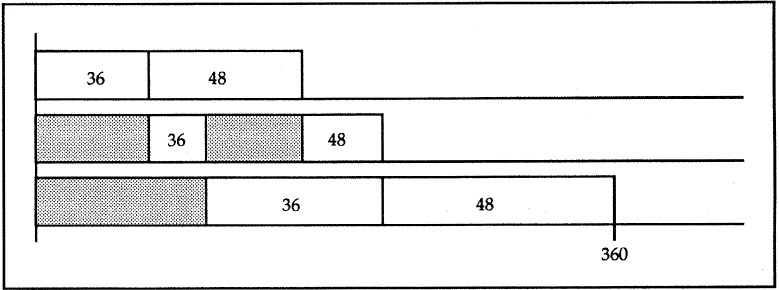
\includegraphics[scale=0.4]{Referencial/Figuras/Ls_ex4}
    \caption{Solução para o exemplo com dois lotes iguais e sem ociosidade}
    \label{fig:LS_ex1}
\end{figure}

        \begin{figure}[!ht]
    \centering
    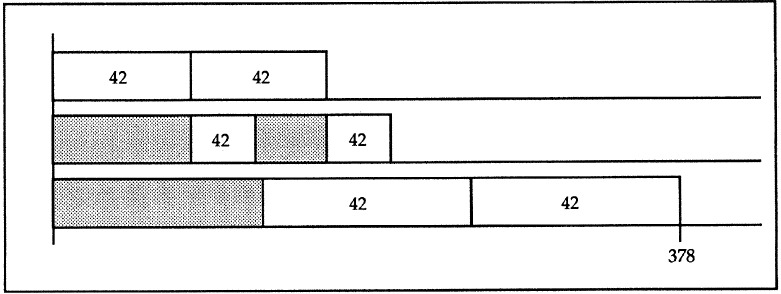
\includegraphics[scale=0.4]{Referencial/Figuras/Ls_ex2}
    \caption{Solução para o exemplo com dois lotes iguais e ociosidade intermitente}
    \label{fig:LS_ex2}
\end{figure}

        \begin{figure}[!ht]
    \centering
    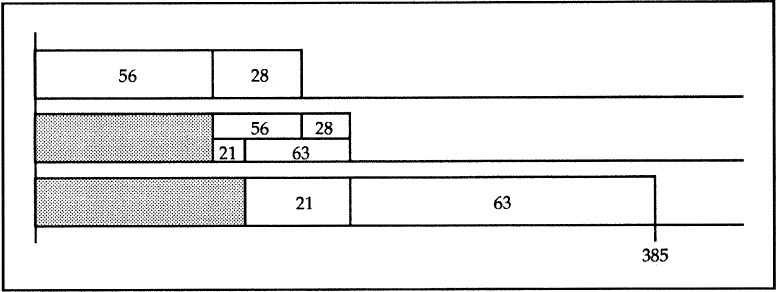
\includegraphics[scale=0.4]{Referencial/Figuras/Ls_ex3}
    \caption{Solução para o exemplo com dois lotes variáveis e sem ociosidade}
    \label{fig:LS_ex3}
\end{figure}

        \begin{figure}[!ht]
    \centering
    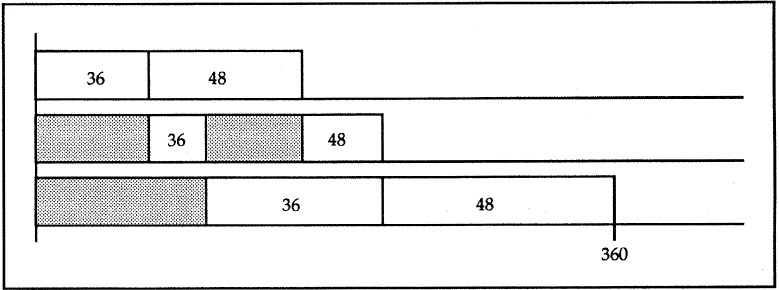
\includegraphics[scale=0.4]{Referencial/Figuras/Ls_ex4}
    \caption{Solução para o exemplo com dois lotes variáveis e ociosidade intermitente}
    \label{fig:LS_ex4}
\end{figure}
        

    \subsection{Simulação de Monte Carlo}
    Segundo \citeonline{CONTE2016}, o método de Monte Carlo é um processo de operações de modelos estatísticos de modo a lidar experimentalmente com variáveis descritas por funções probabilísticas. Esse método baseia-se em um conceito estatístico simples.

    Seja $x$ uma variável aleatória com as seguintes características: função de probabilidade ($f(x)$) e função cumulativa de probabilidades ($F(x)$).
    
    O método de Monte Carlo consiste em:
    \begin{itemize}
        \item Dada a função cumulativa de probabilidades da variável em simulação $F(x)$, toma-se um número, gerado aleatoriamente;
        \item Usando a função cumulativa de probabilidades, determina-se o valor da variável $x$ que corresponde ao número aleatório gerado;
        \item Procedimento de validação que objetiva certificar se a transformação (\textit{input}/\textit{output}) realizada pelo modelo tem a mesma ocorrência procedida no sistema real. Utiliza-se a validação as medidas de posição, dispersão, coeficiente de correlação amostral e testes de hipóteses estatísticas.
    \end{itemize}
    